\documentclass{article}
\usepackage[spanish]{babel}
\usepackage[a4paper,top=2.54cm,bottom=2.54cm,left=2.54cm,right=2.54cm,marginparwidth=1.75cm]{geometry}
\usepackage{amsmath}
\usepackage{graphicx}
\usepackage{listings}
\usepackage{pgfplots}
\usepackage{xcolor}
\usepackage{algorithm} 
\usepackage{algpseudocode} 
\usepackage{pgf-pie}
\usepackage{enumitem}
\definecolor{python_color}{RGB}{255, 99, 71} % Color naranja para Python
\definecolor{cpp_color}{RGB}{65, 105, 225}   % Color azul para C++
\definecolor{pastelblue}{RGB}{102, 153, 204}
\definecolor{pastelred}{RGB}{255, 153, 153}
\definecolor{pastelgreen}{RGB}{102, 204, 102}
\definecolor{pastelyellow}{RGB}{255, 255, 153}
\definecolor{pastelpurple}{RGB}{153, 102, 204}
\definecolor{pastelteal}{RGB}{102, 204, 204}
\definecolor{pastelorange}{RGB}{255, 178, 102}
\definecolor{pastelgray}{RGB}{192, 192, 192}
\definecolor{pastellilac}{RGB}{204, 153, 255}
\definecolor{pastelpink}{RGB}{255, 153, 204}
\definecolor{pastellightblue}{RGB}{153, 204, 255}
\definecolor{pastelgold}{RGB}{255, 204, 153}
\definecolor{mician}{RGB}{0, 120, 135}
\definecolor{fucsia}{RGB}{176, 87, 141}
\definecolor{verdeoscuro}{RGB}{0, 100, 0}
\pgfplotsset{compat=1.17}
\lstset{
    language=Python,
    basicstyle=\ttfamily,
    keywordstyle=\color{fucsia},
    commentstyle=\color{verdeoscuro},
    numbers=left,
    numberstyle=\tiny,
    numbersep=5pt,
    breaklines=true,
    frame=single
}

\begin{document}
    \begin{titlepage}
        \centering
        \vspace*{0.5cm}
        \vspace{1cm}
        
\includegraphics[width=0.4\textwidth]{utdt-logo.jpg} \\
        \vspace{1cm}
        \Large{\bfseries{TD V: Diseño de Algoritmos}}\\
        \vspace{0.8cm}
        \Large{Trabajo Práctico 2}\\
        \vspace{0.5cm}
        \text{Primer Cuatrimestre del 2024} \\
        \vspace{6cm}
        
        \Large{Autores:}\\
        \vspace{0.5cm}
        \Large{Aufiero, Catalina}\\
        \vspace{0.2cm}
        \Large{Brusco, Catalina}\\
        \vspace{0.2cm}
        \Large{Castore, Juan Ignacio}\\

        
        \vfill
        
        \large{Junio del 2024}
    \end{titlepage} 

\section{Introducción}
    \vspace{0.5cm}
    En la actualidad, el cambio climático se presenta como uno de los retos más significativos a nivel mundial. En este contexto, el desarrollo y la gestión eficiente de medios de transporte sostenibles se vuelven cruciales para promover su adopción por parte de la población. Los sistemas ferroviarios destacan como una opción viable, debido a su menor impacto ambiental comparado con los medios de transporte que dependen de combustibles fósiles; es decir, tienen un papel esencial en la reducción de emisiones de gases de efecto invernadero y en el impulso hacia una movilidad más sostenible.

    Para que los sistemas ferroviarios sean efectivos, seguros y funcionen de manera eficiente, es indispensable una planificación adecuada. La capacidad de ofrecer servicios de alta calidad es fundamental para mantener a los usuarios existentes y para atraer nuevos. Dentro de la planificación de un sistema ferroviario, se abordan varias etapas claves interrelacionadas entre sí:
    \begin{enumerate}
            \item Definición del cronograma: Esta etapa implica la creación de un horario detallado para los servicios ferroviarios, especificando los tiempos de salida y llegada en cada estación a lo largo del recorrido. 
            \item Circulación de material rodante: Dado el cronograma y la demanda de pasajeros, es crucial determinar cuántos vagones son necesarios y cómo deben ser utilizados durante el día para satisfacer las necesidades del sistema.
            \item Asignación de tripulaciones: Con el cronograma y la distribución del material rodante definidos, se procede a asignar conductores y demás personal
        \end{enumerate}

    Este informe examina en profundidad los flujos en la optimización ferroviaria, enfocándose en cómo se gestionan y optimizan estos flujos para mejorar la eficiencia y la calidad del servicio en los sistemas ferroviarios contemporáneos. La motivación de este análisis surge del caso de la empresa holandesa de trenes Nederlandse Spoorwegen (NS), que en 2007 revolucionó su enfoque al dejar de realizar adaptaciones manuales de su cronograma y adoptar una nueva estructura más avanzada. Esta nueva estructura permitió ajustar mejor la longitud de los trenes al número de pasajeros, mejorar la programación y reducir los retrasos. Como resultado de estos cambios, NS experimentó un aumento significativo en sus ganancias, un crecimiento del 10-15 \% en el número de pasajeros y una notable mejora en la puntualidad, a pesar del incremento en la cantidad de trenes en operación. En este contexto, el informe analizará las estrategias y algoritmos que se utilizan para optimizar estos flujos y lograr tales mejoras en el rendimiento del sistema ferroviario.
    \\
 
\section{Modelo}
    \vspace{0.5cm}
    El objetivo del problema es determinar la cantidad mínima de vagones necesarios para que cada servicio ferroviario pueda satisfacer su demanda de pasajeros y, al mismo tiempo, mejorar la eficiencia y robustez del sistema. Para ello, el problema toma como input los cronogramas de los servicios de dos terminales de tren conectadas, la demanda (es decir, el número de pasajeros) para cada evento (partida o llegada de un tren) y la capacidad de cada vagón, asumiendo una flota homogénea.
    
    Para abordar el problema, se considera que cada tren toma inicialmente los vagones necesarios de un stock disponible (con cantidad infinita) en su estación de origen, realiza su recorrido y finaliza en la estación de destino. Esta visión inicial podría implicar un uso elevado de vagones a lo largo del día. No obstante, se puede optimizar esta utilización mediante una planificación que permita la reutilización eficiente de los vagones entre distintos servicios. Por ejemplo, si un tren llega a una estación antes de que otro salga, los vagones del tren que llega pueden ser reutilizados por el tren que está por partir, lo que reduce la cantidad total de vagones requeridos.
    Este tipo de problemas se conoce como circulación de material rodante, y se resuelven mediante principios de optimización que buscan la asignación más eficiente de recursos. En general, es útil comenzar el día asignando a los primeros servicios de cada terminal el número mínimo de vagones necesarios y planificar la reutilización de estos vagones entre los trenes a lo largo del día. Si es necesario, se pueden agregar vagones adicionales para cubrir la demanda.
    
    El problema presenta ciertas reglas:
    \begin{enumerate}
     \item \textbf{Uso uniforme de unidades}: Todos los servicios emplean el mismo tipo de unidad de tren, y esta unidad es única para todo el sistema.
    \item \textbf{Transferencias de unidades entre servicios}: Un servicio puede transferir unidades a uno o más servicios posteriores, que pueden no ser necesariamente los que salen inmediatamente después, siempre y cuando el traspaso ocurra en la misma estación.
    \item \textbf{Transferencias parciales}: Las unidades pueden transferirse de manera parcial entre los servicios; no es necesario que el traspaso sea de todas las unidades.
    \item \textbf{Almacenamiento temporal}: Las unidades que no se usan en una estación se almacenan temporalmente en el patio de maniobras. Para simplificar, se asume inicialmente que este patio tiene una capacidad infinita.
    \item \textbf{Satisfacción de la demanda}: La cantidad de unidades asignadas a un servicio debe ser suficiente para satisfacer la demanda de pasajeros. Es posible asignar más unidades de las necesarias para facilitar su reubicación.
    \item \textbf{Restricciones de infraestructura}: Los servicios tienen una limitación en el número máximo de unidades que pueden operar simultáneamente, debido a restricciones de la infraestructura.
    \item \textbf{Transferencias solo en estaciones clave}: En el contexto operativo de la empresa, las unidades solo pueden transferirse entre servicios en las estaciones principales o cabeceras.
    \item \textbf{Final del día}:Al finalizar el día, ambas estaciones cuentan con la misma cantidad de unidades que al inicio,
 puediendo repetir la misma asignación. 
    \end{enumerate}

     

    
    Este modelo se representará como un grafo dirigido, específicamente definido como un grafo $G = (V, A)$ (ver Figura 1 y 2), donde:

    \begin{enumerate}
    \item El conjunto de \textbf{vértices} $V$ contiene un nodo para cada evento en cada servicio, es decir, cada llegada o partida de un tren se representa como un vértice distinto.
    \item El conjunto de \textbf{aristas} $A$ se compone de tres tipos diferentes de conexiones:
    \begin{enumerate}
        \item \textbf{Aristas de tren}: Estas aristas $(i, j)$ conectan el evento de partida de un servicio con su correspondiente evento de llegada, representando el trayecto del tren desde la estación de origen hasta la estación de destino. Cada una de estas aristas tiene una cota inferior $l_{ij}$, que indica el número mínimo de unidades (vagones) necesarios para satisfacer la demanda, y una cota superior $u_{ij}$, que representa la cantidad máxima de unidades que pueden operar en el servicio. Para simplificar, asumimos que $u_{ij}$ es la misma para todos los servicios. El costo asociado a estas aristas es $c_{ij} = 0$.
        \item \textbf{Aristas de traspaso}: Estas aristas $(i, j)$ conectan dos eventos consecutivos en el tiempo dentro de una misma estación, facilitando la transferencia de unidades de un tren a otro. En este caso, la cota inferior $l_{ij} = 0$, la cota superior $u_{ij} = \infty$, y el costo $c_{ij} = 0$.
        \item \textbf{Aristas de trasnoche}: Estas aristas $(i, j)$ conectan el último evento del día en una estación con el primer evento del día siguiente, representando la continuidad de las operaciones y la necesidad de que las unidades estén en su lugar al final del día para iniciar las operaciones del día siguiente. Inicialmente, tienen una cota inferior $l_{ij} = 0$, una cota superior $u_{ij} = \infty$, y un costo $c_{ij} = 1$. La cantidad total de unidades necesarias para el sistema se obtiene sumando el número de unidades que circulan por estas aristas de trasnoche.
    \end{enumerate}
    \end{enumerate}

    Dado que se trata de un problema de circulación, el balance de flujo en todos los vértices debe ser cero. Sin embargo, las cotas inferiores en las aristas de tren permiten reflejar la necesidad mínima de unidades para satisfacer la demanda de pasajeros.

    El modelo propuesto aborda una asignación eficiente de recursos y la satisfacción de la demanda en sistemas ferroviarios. Al considerar diversos eventos y establecer cotas para la circulación de material rodante, este enfoque permite mejorar la eficiencia operativa y la calidad del servicio, contribuyendo así al desarrollo de sistemas de transporte más eficientes y sostenibles.

    
     

\begin{figure}[htbp]
    \centering
    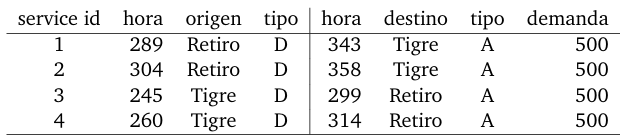
\includegraphics[width=0.5\textwidth]{imagenhorarios.png}
    \caption{Ejemplo de un cronograma con 4 servicios entre Tigre y Retiro}
    \label{fig:ejemplo}
\end{figure}

\begin{figure}[htbp]
    \centering
    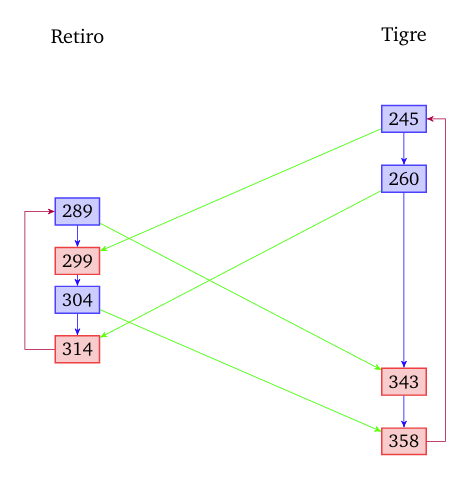
\includegraphics[width=0.5\textwidth]{grafo.png}
    \caption{Ejemplo de un cronograma con 4 servicios entre Tigre y Retiro}
    \label{fig:ejemplo}
\end{figure}

    \section{Implementación}
    \vspace{0.5cm}
    \subsection{Flujo Máximo a menor costo}
        
    Al implementarlo, optamos por utilizar Python junto con algunas bibliotecas clave como Networkx para la manipulación de grafos, matplotlib y math. Comenzamos tomando como entrada los servicios disponibles entre dos estaciones de tren y creamos un grafo dirigido para representar esta red.
    
    En este grafo, cada nodo de partida está asociado con la información del servicio de tren, que incluye horario, tipo de servicio y origen; estructurado de esta manera para evitar referirnos erróneamente a un nodo cuando existen al menos dos nodos con mismo horario pero de diferentes estaciones. Cada nodo está dirigido a: el nodo del servicio de llegada -con la misma estructura de representación-; y con el próximo tren posterior a él en su misma estación, las especificaciones estan detalladas en la sección del modelo.
    
   Al recorrer todos los servicios, los agrupamos según la estación en Conjuntos para evitar repeticiones, y posteriormente los convertimos en Listas para facilitar su ordenamiento ascendente según la hora.
    
    Para resolver el problema de  máximo flujo con menor costo, fue crucial  ajustar el flujo, es decir, equilibrar las demandas y capacidades de los nodos y aristas respectivamente, antes de aplicar el algoritmos. Esto implicó ajustar ciertos atributos de los nodos, como las demandas, calculando la diferencia entre el flujo que egresa y lo que ingresa en cada nodo. Además, modificamos atributos de los arcos, estableciendo un límite inferior de 0 y ajustando las capacidades para reflejar la diferencia entre la capacidad máxima permitida y el límite inferior.
    
    Estos ajustes permitieron modelar correctamente el problema y aplicar el algoritmo para encontrar la solución óptima bajo las condiciones, en otras palabras, la menor cantidad de vagones para una determinada instancia.

     Aclaración: Para realizar pruebas exhaustivas, hemos desarrollado el script \texttt{prueba.py}, el cual puede generar múltiples instancias con servicios creados de manera aleatoria. Este script acepta como parámetro la cantidad de servicios que se desean generar.
     También desarrollamos un graficador simple para obtener una representación visual del grafo cuando se generan instancias pequeñas, dado que con un gran número de servicios el grafo tiende a volverse ilegible.


    \subsubsection{Pseudocódigo}
    Figura 3 y 4 al final del documento.
    \subsubsection{Flujo máximo con una mejor solución que un algoritmo goloso}
       
    Este ejercicio se baso en comparar el algoritmo goloso que utiliza la empresa con el que planteamos nosotros del costo mínimo del flujo máximo. A primera vista, parecía que ambos eran eficientes y llegaban a la misma respuesta. Luego de observar y experimentar un tiempo, nos terminamos dando cuenta que había una serie de casos donde el flujo daba una respuesta más óptima que la que daba el algoritmo de la empresa. Esto sucede cuando en algún viaje es conveniente llevar más vagones que los que se necesitarían para cubrir la demanda, ya que estos serían necesitados en algún viaje próximo y así evitar que se sumen a la cantidad de vagones que se necesitan. En otras palabras, el algoritmo de la empresa siempre va a hacer viajes con la cantidad de vagones exacta que se necesitan, mientras que el algoritmo que planteamos nosotros de flujo máximo tiene en cuenta otros escenarios, el de los proximos viajes, y puede ver cuál va a ser la cantidad óptima de vagones en base a esto. Buscamos dos casos dónde esto sucedía:
    
    \subsubsection{Ejemplo 1}

\begin{figure}[h!]
    \raggedright
    \centering

    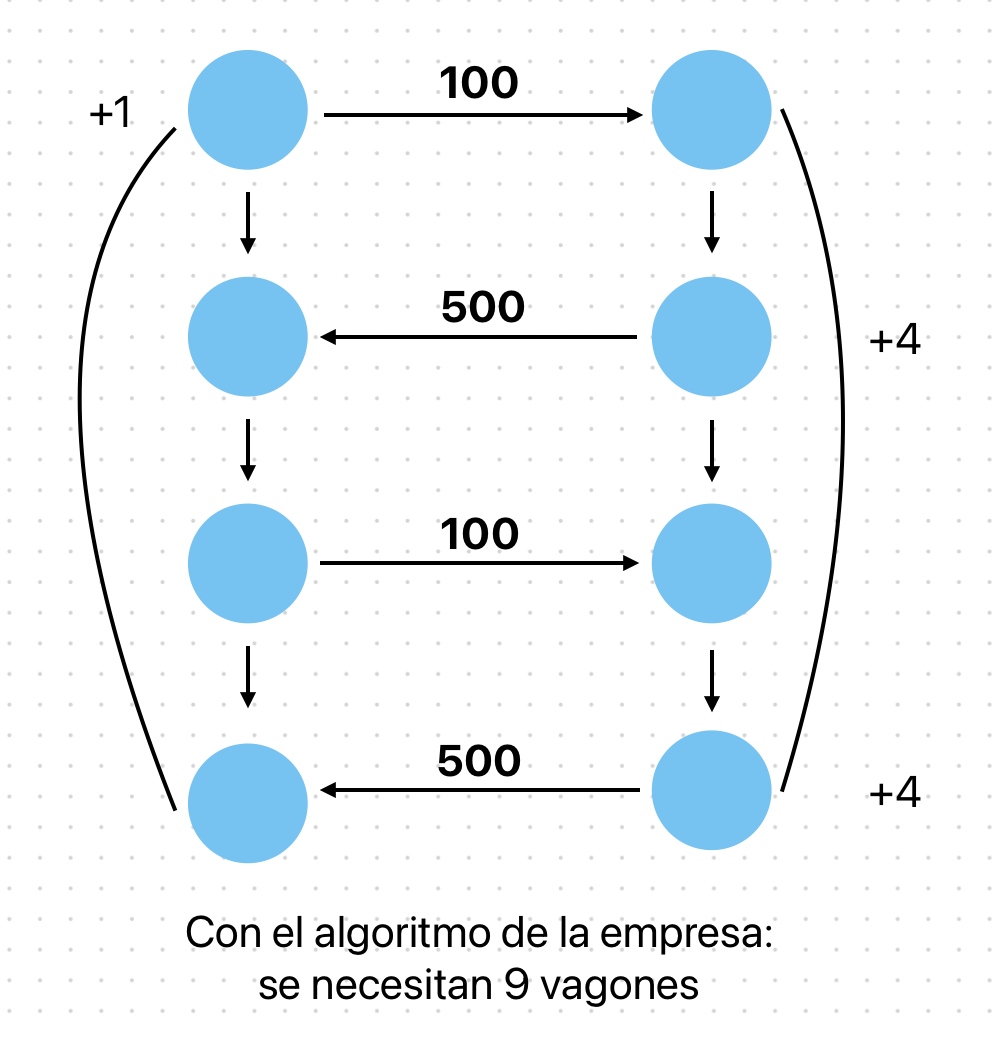
\includegraphics[scale=0.35]{im1.png}
    \caption{Ejemplo 1}

    \label{fig:ejemplo}
\end{figure}

En este ejemplo podemos ver como con el algoritmo de la empresa se necesitan en total 9 vagones (son los +1 y +4 que están al costado de los nodos). Luego, cuando probamos este mismo caso en el algoritmo nuestro, en la instancia "./instances/ejercicio2.json" vemos cómo pasamos de necesitar 9 vagones a necesitar solamente 5. Esto es un ejemplo de lo que expusimos antes, donde el algoritmo de la empresa manda exactamanete tantos vagones como los que osn demandados, mientras que en el flujo máximo, cambiaría que en la tercera arista (mirandolas de arriba para abajo), en vez de enviar 1 vagón, estarían enviando 5 (los 5 que recién llegaron), que luego serían utilizados para el último viaje que se necesitan 5 vagones, y acá estarían evitando pedir 4 vagones más. 

\subsubsection{Ejemplo 2}

\begin{figure}[h!]
    \raggedright
    \centering

    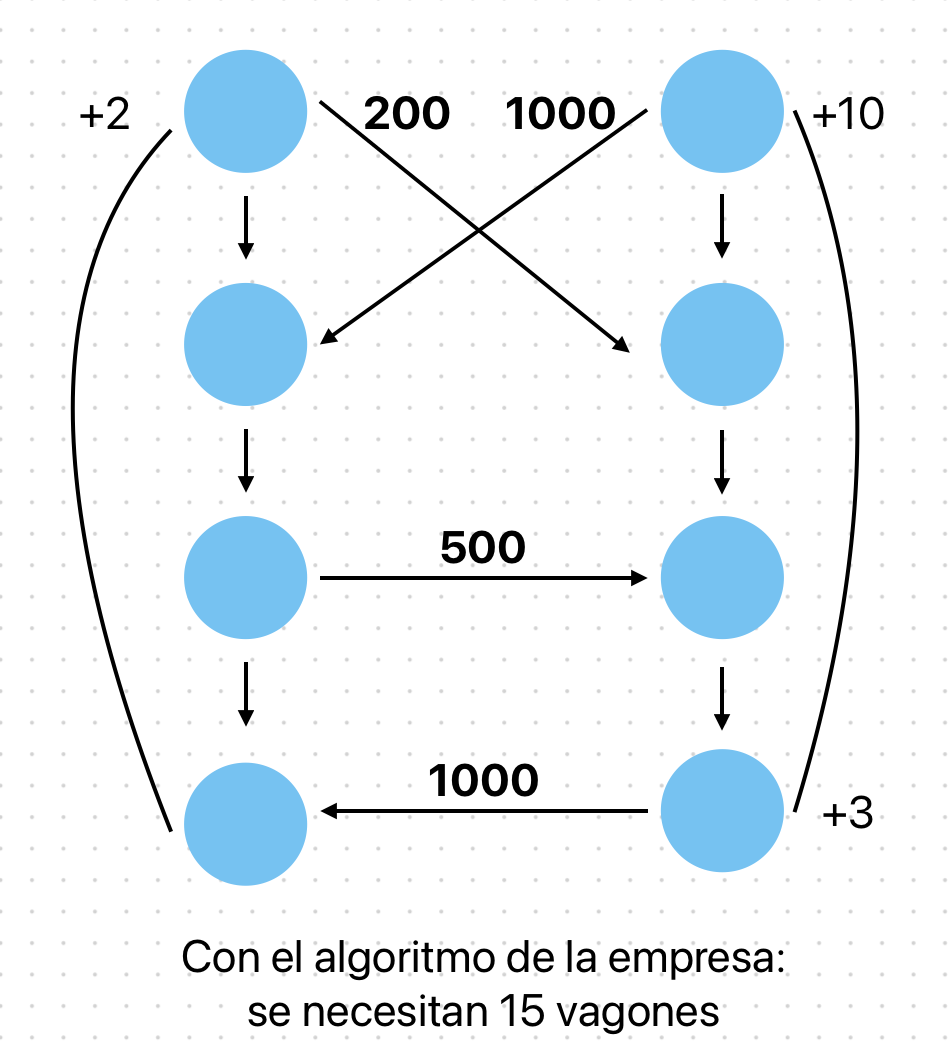
\includegraphics[scale=0.35]{im2.jpg}
    \caption{Ejemplo 2}

    \label{fig:ejemplo}
\end{figure}

Este es otro ejemplo que sucede esto mismo, donde el algoritmo que proporciona la empresa no termina de ser el más eficiente. Como podemos ver con los +  a los costados de los nodos, la empresa estaría en total utilizando 15 vagones. En cambio, con el algoritmo propuesto por nosotros, se estarían utilizando 12 vagones ya que en la tercera arista (mirando desde arriba hacia abajo) podríamos mandar 10 vagones y esos 10 ultilizarlos para el último viaje, y así usando 3 vagones menos en total. Vale la pena aclarar que todos estos ejemplos es suponiendo que la capacidad de cada vagón es de 100.
    

\vspace{2cm}

\section{Experimentación}
\vspace{0.5cm}
       Resultó interesante modificar las demadas de los servicios que se utilizan en el horario actual de Tigre-Retiro. Lo anterior se debe a que en Argentina es frecuente que algún servicio se vea inhabilitado un día, ya sea por paros o manifestaciones, y por lo tanto la cantidad de personas que utilizaba el transporte perjudicado se distribuye en los pocos transportes que restan disponibles. 

      \begin{table}[htbp]
        \centering
        \caption{Aumento de demanda y utilización de vagones en la ruta Tigre-Retiro}
        \begin{tabular}{|c||c|c|c|c|c|c|c|c|c|c|c|}
            \hline
            \textbf{Variac. de Demanda} & \textbf{0\%} & \textbf{10\%} & \textbf{20\%} & \textbf{30\%} & \textbf{40\%} & \textbf{50\%} & \textbf{60\%} & \textbf{70\%} & \textbf{80\%} & \textbf{90\%} & \textbf{100\%} \\
            \hline
            \textbf{Cant. de Vagones}   & 48           & 56           & 56           & 64           & 64           & 72           & 79           & 80           & 88           & 88           & 96            \\
            \hline
            \textbf{Variac. de Vagones}          & -            & +8           & 0            & +8           & 0            & +8           & +7           & +1           & +8           & 0            & +8            \\
            \hline
        \end{tabular}
    \end{table}

    En el Cuadro 1 podemos observar los resultados, mostrando cómo la variación en la demanda afecta la utilización de vagones en la ruta Tigre-Retiro. A medida que la demanda aumenta, observamos un incremento en la cantidad de vagones utilizados, aunque este aumento no es completamente lineal. Para incrementos iniciales del 0\% al 10\%, el número de vagones aumenta de 48 a 56, indicando que el sistema puede absorber pequeñas variaciones sin necesidad de ajustes inmediatos (es decir, agregar vagones). Sin embargo, con ciertos incrementos de demanda (en los casos de 20\%, 40\% y 90\% de aumento) la cantidad de vagones no se ve incrementada; a diferencia de los casos restantes que requieren un incremento significativo de vagones, como de 20\% a 30\%, donde se requieren 8 vagones adicionales ya que pasa de 56 a 64. A su vez, resulta llamativo el incremento de sólo 1 vagón cuando la demanda sube del 60\% al 70\%, reflejando ajustes casi insignificativos para acomodar la demanda adicional. Es interesante notar que existe un patrón en la cantidad de vagones incrementados: suelen ser 8 vagones o 0 vagones, a exepción del caso que sólo aumenta uno. Lo anterior nos motivó a querer observar si pasaba lo mismo reduciendo las demandas, en vez de incrementandolas (Cuadro 2).
    \begin{table}[htbp]
            \centering
            \caption{Decremento de demanda y utilización de vagones en la ruta Tigre-Retiro}
            \begin{tabular}{|c||c|c|c|c|c|c|c|c|c|c|c|}
                \hline
                \textbf{Variac. de Demanda} & \textbf{0\%} & \textbf{10\%} & \textbf{20\%} & \textbf{30\%} & \textbf{40\%} & \textbf{50\%} & \textbf{60\%} & \textbf{70\%} & \textbf{80\%} & \textbf{90\%} & \textbf{100\%} \\
                \hline
                \textbf{Cant. de Vagones}   & 48           & 48    & 40       & 32           & 32           & 24           & 24           & 16           & 16           & 8           & 0                  \\
                \hline
                \textbf{Variac. de Vagones} & - & 0 & -8 & -8 & -8 & -8 & 0 & -8 & 0 & -8 & -8\\
                \hline
            \end{tabular}
        \end{table}
        Nuevamente, el Cuadro 2 muestra una relación directa entre la variación en la demanda y la cantidad de vagones utilizados en la ruta. A medida que la demanda comienza a disminuir, por ejemplo, en un 10\%, la cantidad de vagones se mantiene en 48, indicando una capacidad inicial que no necesita ser ajustada inmediatamente.
        
        Sin embargo, a medida que la demanda continúa disminuyendo, hay una reducción gradual en la cantidad de vagones utilizados. Cuando la demanda cae un 20\%, la cantidad de vagones se reduce a 40, lo que representa una disminución de 8 vagones respecto al escenario inicial. Esta reducción se intensifica a medida que la demanda sigue bajando: un descenso del 30\% resulta en 32 vagones, y así sucesivamente.

        A la hora de comparar ambos escenarios, es importante destacar ciertos aspectos. Primero, ambos tienen las mismas variaciones absolutas de vagones,es decir 8 o ninguna (excluyendo el caso de aumento en 1 y de 7 vagón del Cuadro 1); podría deberse a que modificamos la base de datos en la misma proporción (en saltos de 10\%), sólo que en un caso se incrementa y en el otro se decrementa. Segundo, nos gustaría mencionar que en el CUadro 1 tenemos dos escenarios que no se dan en el Cuadro 2, que es incrementar en 7 vagones o incrementar en 1 vagón; nos llamó la atención que estos valores no se vean reflejados en algún momento al decrementar la demanda.

        De cualquier manera, ambos cuadros ilustran cómo la gestión de recursos, específicamente la cantidad de vagones, puede variar significativamente según si la demanda está aumentando o disminuyendo. En cada escenario se implementa la solución con mayor flujo y mínimo costo adaptando la cantidad de vagones, asegurando una respuesta efectiva a las necesidades cambiantes de los usuarios y manteniendo la operación eficiente del servicio.

    Otro experimento interesante de llevar acabo fue notar la sensibilidad del costo frente a demoras o adelantos de los horarios muy pequeñas. A priori, pensabamos que aumentar atrasar en un minuto un servicio, no repercutiría demasiado en el costo en términos de vagones; pero el resultado fue opuesto. Observemos cómo modificando sólo en una cierta cantidad de minutos la llegada del servicio, se puede ver perjudicado el costo. 

    \begin{table}[htbp]
            \centering
            \caption{Retraso del servicio y utilización de vagones en la ruta Tigre-Retiro}
            \begin{tabular}{|c||c|c|c|c|c|c|c|c|c|c|c|}
                \hline
                \textbf{Retraso (en minutos)} & \textbf{0} & \textbf{1} & \textbf{2} & \textbf{3} & \textbf{4} & \textbf{5} & \textbf{6} & \textbf{7} & \textbf{8} & \textbf{9} & \textbf{10} \\
                \hline
                \textbf{Cant. de Vagones}   & 48           & 48    & 54       & 54           & 54           & 54           & 59           & 59           & 59           & 60           & 60                  \\
                \hline
                \textbf{Variac. de Vagones} & - & 0 & +6 & 0 & 0 & 0 & +5 & 0 & 0 & +1 & 0\\
                \hline
            \end{tabular}
        \end{table}
       En el Cuadro 3 se observa cómo los retrasos en el arribo del servicio impactan la cantidad de vagones necesarios para mantener el funcionamiento eficiente de la ruta Tigre-Retiro. Por ejemplo, un retraso de 2 minutos en la llegada del tren requiere la utilización de 6 vagones adicionales, mientras que un retraso de 6 minutos implica la necesidad de 11 vagones más, y un retraso de 10 minutos requiere 12 vagones adicionales. 
       La necesidad de aumentar el número de vagones en respuesta a los retrasos está directamente relacionada con la capacidad de la empresa para gestionar el flujo de pasajeros y mantener la calidad del servicio. Cada minuto de retraso en la llegada del tren provoca una acumulación de pasajeros que debe ser gestionada en el próximo servicio con una mayor cantidad de vagones. 
       
       Cuando modelamos este problema, es crucial reconocer que los retrasos no solo afectan la puntualidad del servicio, sino que también tienen implicaciones significativas en los costos operativos de la empresa. El aumento en la cantidad de vagones conlleva mayores gastos. Por lo tanto, un retraso de 2 minutos, que implica la utilización de 6 vagones adicionales, representa un incremento considerable en los costos para la empresa. Este incremento es aún más pronunciado con retrasos mayores, como los de 6 y 10 minutos.
       
        Dicho experimento se implementó con los servicios de Tigre-Retiro donde ya dos minutos de retraso en la llegada del tren, repercute en el costo; mencionamos esto porque en el caso de que cada tren partía cada 20 minutos, el costo no se hubiera visto afectado, sería el mismo que el inicial. 
        Es importante mencionar que en este análisis se consideran los trenes de la instancia Tigre-Retiro, donde a partir de los dos minutos de retraso, ya hay un impacto significativo en el costo total. Si tomabamos una instancia donde cada tren partía cada 20 minutos, el impacto del retraso en el costo, sería nulo ya que en el peor caso se retrasaría 10 minutos, pero aún así no alteraría el resto de los servicios. En otras palabras, con intervalos de partida más largos, la necesidad de ajustar la cantidad de vagones en respuesta a pequeños retrasos podría ser menos pronunciada, ya que la acumulación de pasajeros sería menor en comparación con intervalos de partida más cortos.
        \vspace{1cm}
        
\textbf{Situación 4}
\newline
    Otro experimento que hicimos, fue ver la diferencia entre dos escenarios: el primero sería el caso donde todos los viajes llevan la misma cantidad de vagones tal que en todos los viajes la demanda sea cubierta. Este caso se encuentra en "./instances/experimentacion-c.json" donde la demanda de cada viaje es 700 (cubriría todas las demandas originales). En este caso el costo minimo es de 42 vagones. 
    Después de esto quisimos ver que pasaba si poníamos los valores originales en las demandas, donde el algoritmo creado comienza a tener más sentido, ya que busca utilizar la menor cantidad de vagones nuevos mientras que se cumpla la demanda. Acá el costo mínimo nos dió de 30 vagones. Esto se encuentra en "./instances/experimentacion-c2.json". 
    Gracias a este experimento, podemos afirmar que el algoritmo intenta optimizar lo máximo posible con el fin de utilizar la menor cantidad de vagones.

\vspace{1cm}

\textbf{Situación 5}
\newline
    En un escenario donde la hora pico se alcanza a los 120 minutos del día con una demanda de 1000 pasajeros viajando de Retiro a Tigre, realizamos un experimento para evaluar los efectos de cambiar ese único tren a los 120 minutos por tres trenes con capacidad para 333 pasajeros cada uno, programados para los minutos 100, 120 y 140. Aplicamos la misma estrategia para el tren de Tigre a Retiro, que también tiene una demanda de 1000 pasajeros a los 100 minutos. Este tren se dividió en tres trenes con una capacidad de 333 pasajeros cada uno, programados para los minutos 90, 110 y 130. 

    El objetivo de esta reestructuración fue intercalar los trenes de ambos trayectos para maximizar el uso de los vagones disponibles, reduciendo la necesidad de utilizar vagones adicionales. Las dos instancias del experimento se documentaron en los archivos "./instances/experimentacion-c3.json" y "./instances/experimentacion-c4.json".

    Después de calcular los costos y analizar los resultados, observamos que en el esquema original se requerían 33 vagones. Sin embargo, con la modificación implementada, solo se necesitaron 17 vagones. Esto demuestra una optimización significativa y una reducción en el número de vagones necesarios, gracias a la reutilización eficiente de los mismos.
\vspace{0.5cm}

\textbf{Situación 6}
\newline
    Teníamos la hipótesis de que el costo del flujo de servicios no depende simplemente de la cantidad total de servicios, sino más bien de la distribución de estos servicios y de la demanda específica asociada a cada uno. Por ejemplo, si disponemos de 100 servicios, todos con una demanda de 500 unidades y organizados de manera que se optimice el uso de los vagones, podríamos satisfacer todas las demandas con tan solo 5 vagones. En contraste, si tenemos 4 servicios con una demanda total de 1000 unidades y están organizados de manera ineficiente, como con dos servicios saliendo desde una estación y luego dos desde otra, el costo sería mucho mayor, a pesar de haber transportado menos personas y realizado menos viajes en total.

    Pudimos verificar esta hipótesis utilizando el script \texttt{experiment.py}, donde generamos un cronograma con un ordenamiento eficiente y una gran cantidad de servicios (todos con demanda de 500 unidades). Observamos que el número de vagones necesarios oscilaba entre 5 y 10, convergiendo en estos valores. Esto sugiere que podríamos teóricamente gestionar cronogramas con una cantidad infinita de servicios, aunque en la práctica esto sería inviable.

    En la imagen numero 5 se puede observar la validación de esto. Además, este gráfico se puede obtener ejecutando el script mencionado.

    La conclusión es que podemos reducir el costo del cronograma ajustando la cantidad total de servicios a un número par y organizándolos de manera eficiente para maximizar la reutilización de los vagones.

\begin{figure}[h!]
    \raggedright
    \centering

    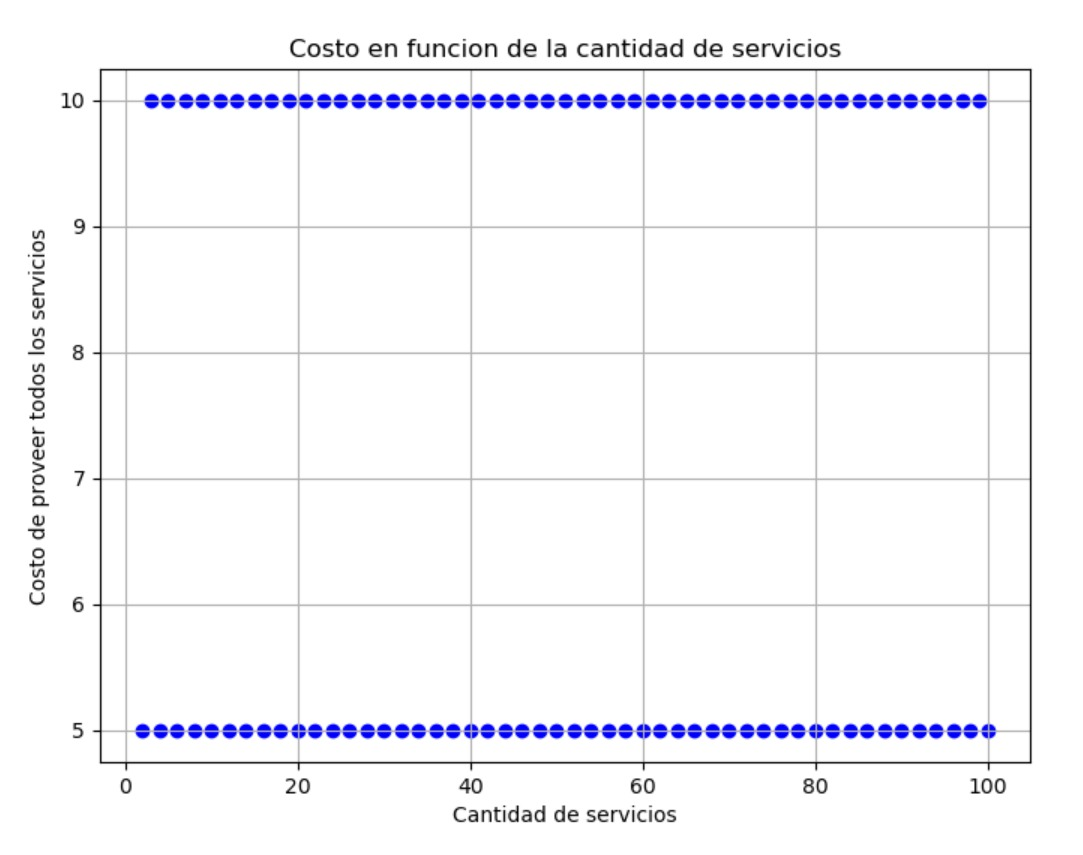
\includegraphics[scale=0.35]{costoXServicios.jpeg}
    \caption{Costo por cantidad de servicios}

    \label{fig:ejemplo}
\end{figure}

\section{Nuevo escenario}
    Para abordar el problema de la restricción en el almacenamiento de vagones debido a futuros trabajos de infraestructura en una de las estaciones terminales, se deben realizar ajustes específicos en el modelo de planificación.
    Se prevé que, debido a las obras en la infraestructura, una de las estaciones terminales tendrá una limitación en el número de vagones que pueden permanecer allí durante la noche. Esta capacidad limitada será conocida con antelación. Para integrar esta nueva restricción en el modelo y adaptarlo adecuadamente, se propone una metodología específica.
    En la estación afectada, donde no se podrán almacenar vagones, añadiremos una dos un nuevo camino que esta compuesto por 2 arcos y un nodo intermedio (por limitaciones de Networkx). Estas aristas conectarán el último nodo de la estación afectada con el primer nodo de la estación afectada pasando por el nodo intermedio. Este nodo intermedio representa un lugar alternativo donde los vagones pueden ser almacenados temporalmente.
    Al incorporar este nuevo camino, es necesario asignarle un costo superior, para que forzar que el flujo primero agote la capacidad de la arista de trasnoche inicial. De esta manera, el sistema prioriza la ruta más económica y eficiente hasta que sea absolutamente necesario desviar el flujo, que serán la cantidad de vagones que necesitan reubicarse.
    
    \vspace{6cm}
    
\begin{figure}[h!]
    \raggedright
    \centering

    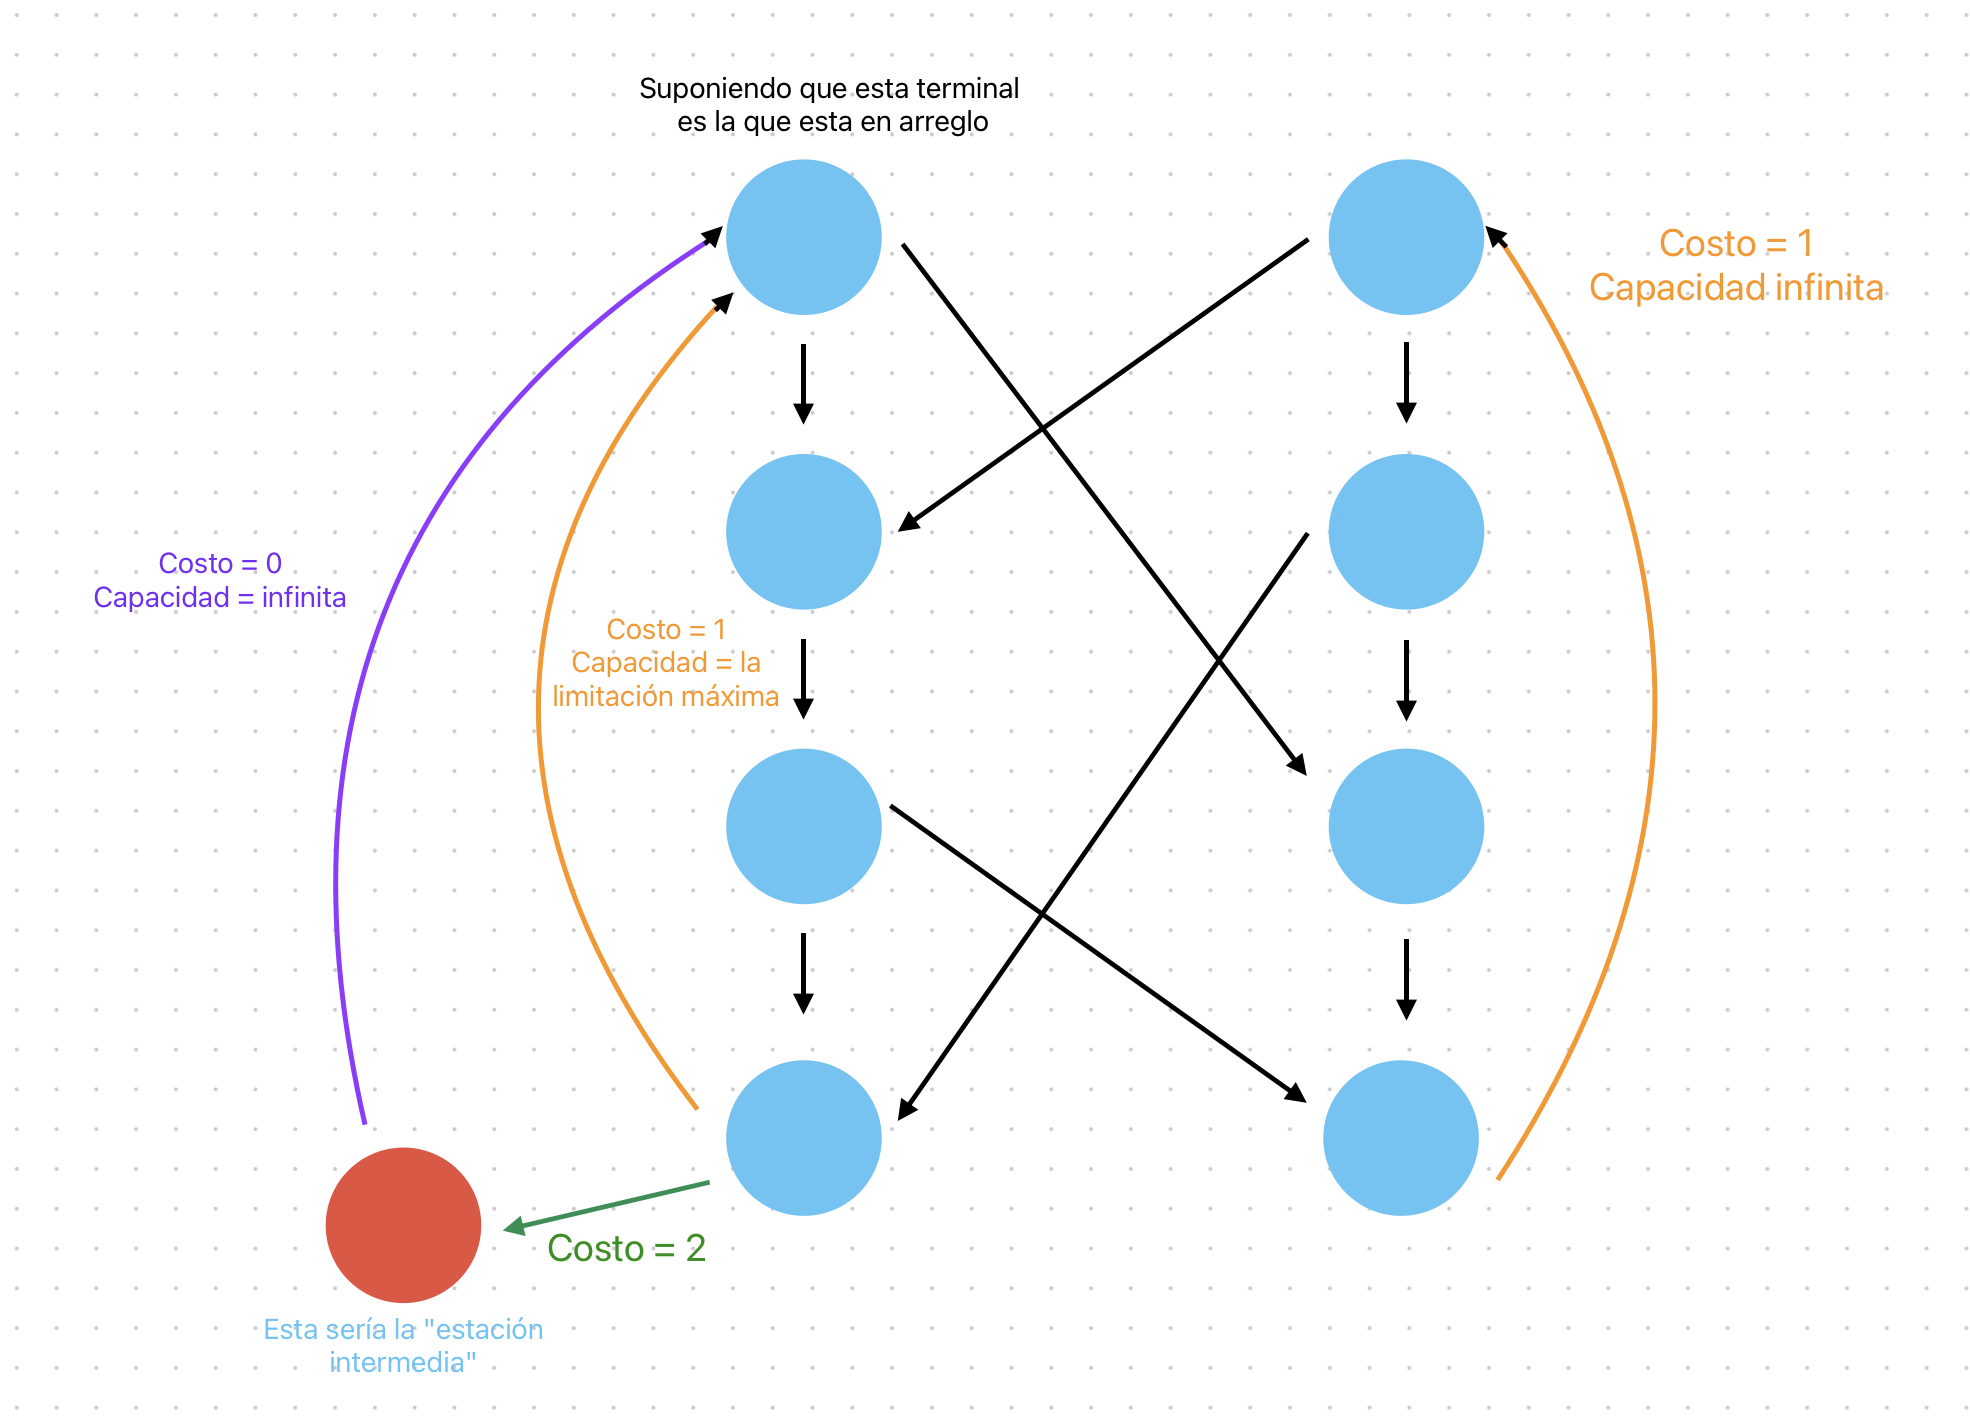
\includegraphics[scale=0.35]{ejercicio5.png}
    \caption{Escenario Adicional Ejemplo}

    \label{fig:ejemplo}
\end{figure}






    
\section{Conclusión}
    \vspace{0.5cm}
    El problema de la circulación de material rodante consiste en determinar cuántas unidades asignar a cada servicio de tren para satisfacer la demanda y cómo realizar los traspasos entre ellos para minimizar el número total de vagones necesarios. Este desafío puede abordarse eficazmente mediante el algoritmo de máximo flujo con menor costo. Este enfoque permite optimizar la asignación de recursos, asegurando que los servicios de tren operen de manera eficiente y rentable.

Además, una variación del modelo original que considera situaciones donde una de las estaciones terminales tiene restricciones en la capacidad de almacenamiento de vagones resulta crucial para materializar el problema. Este algoritmo es vital porque una empresa de transporte decide diariamente cómo asignar sus recursos, lo que influye directamente en sus ganancias.

Tras experimentar con diversos escenarios, hemos observado que la cantidad mínima de vagones necesaria está estrechamente relacionada con los intervalos de partida de los trenes. Sin embargo, en ocasiones, enviar la mínima cantidad de vagones no siempre resulta ser la mejor decisión desde una perspectiva operativa y económica. Muchas veces, realizar más viajes puede resultar en una asignación más eficiente. Esto puede parecer contraintuitivo, ya que es natural pensar que al hacer más viajes se incurre en mayores costos, cuando en realidad, aunque se consume más energía en el viaje, también se ahorra en la cantidad de trenes necesarios para cumplir con la demanda.

Resultaría interesante analizar si unificar dos servicios en caso de retrasos podría potencialmente mejorar los resultados. La optimización de la circulación de material rodante es fundamental para la eficiencia y la rentabilidad del servicio ferroviario, y la aplicación de algoritmos avanzados como el de máximo flujo con menor costo ofrece soluciones para enfrentar este desafío.

Cabe destacar que nuestro modelo es una versión muy simplificada de la realidad, donde mostramos la idea principal de asignar recursos de manera eficiente. Sin embargo, para poder realizar este modelado, hemos dejado de lado muchas variables que en la vida real deberían ser consideradas. Entre estas variables se encuentran: la capacidad máxima de vagones que pueden estar en una estación, así como la capacidad total de la empresa (pues podría darse el caso de que el número total de vagones no sea suficiente para satisfacer la demanda y se deba buscar la manera de cumplir la mayor demanda posible con los vagones disponibles). También, hay ciertos escenarios infactibles, como por ejemplo, tener todos los servicios de una estación cabecera a otra, pero ninguna de la segunda a la primera. 

Otras variables que deberían tenerse en cuenta incluyen la cantidad máxima de vagones que puede haber en una vía al mismo tiempo, la distancia "segura" entre dos trenes, la existencia de vagones de distintas capacidades (lo que requeriría distinguir entre tipos de vagones), y la falta de intersecciones en las vías donde un tren podría cambiar de ruta, así como la ausencia de estaciones intermedias, trabajando solo con dos estaciones en cada extremo de una única vía del tren.
    \begin{figure}[htbp]
    \centering
    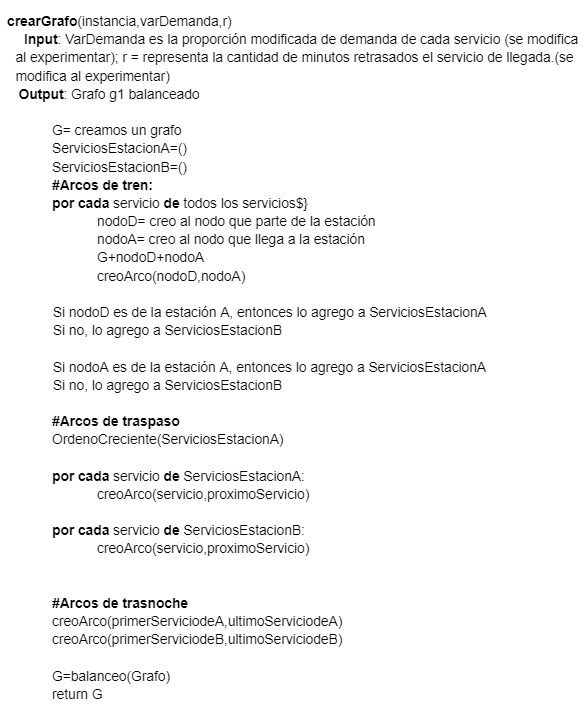
\includegraphics[width=0.5\textwidth]{imagen_pseudo.png}
    \caption{Función Crear grafo}

    \label{fig:ejemplo}
    \end{figure}
    \begin{figure}[htbp]
    \centering
    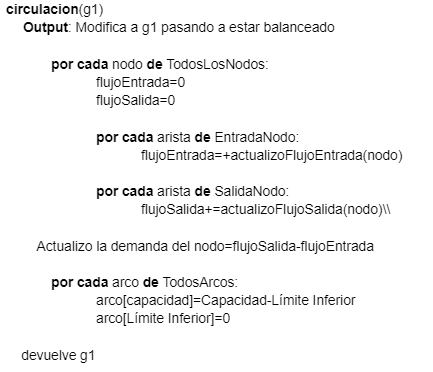
\includegraphics[width=0.5\textwidth]{image.png}
    \caption{Función Circulación}

    \label{fig:ejemplo}
    \end{figure}
        
\end{document}

El modelo,
 la descripción de los modelos y algoritmos, las decisiones de diseño, la implementación,
 el testing realizado, la presentación de resultados, instrucciones de compilación y ejecución.